\documentclass{article}%set file type

\usepackage{tikz}
\usetikzlibrary{arrows,automata}%use arrows lib, plot arrow, use automata lib, plot AC


\definecolor{shadecolor}{rgb}{0.95,0.95,0.95}
\pagecolor{shadecolor}
\begin{document}

	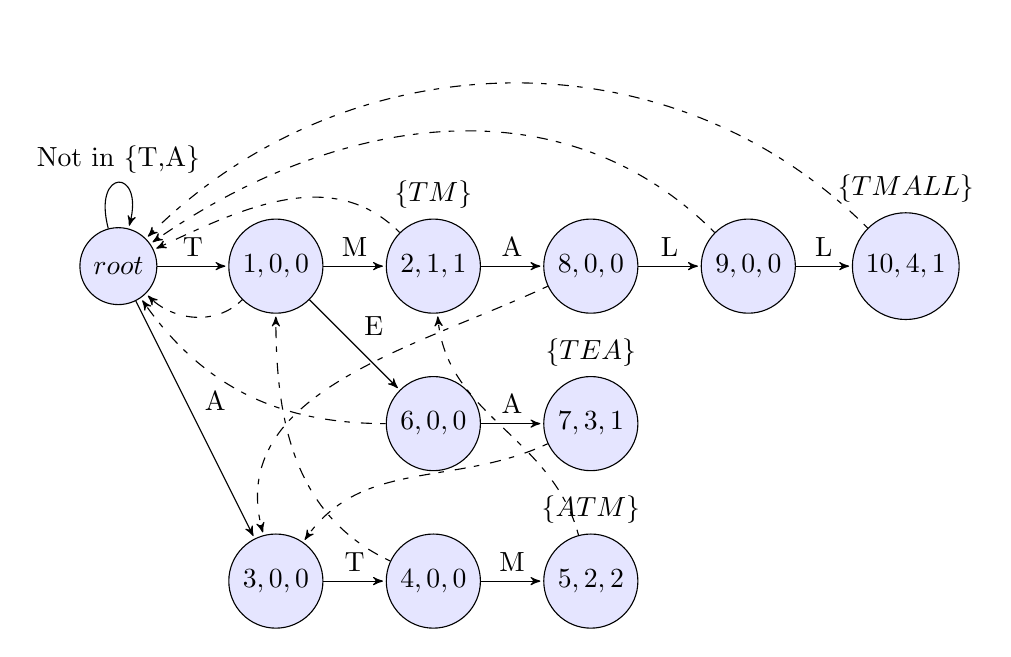
\begin{tikzpicture}[shorten >=1pt,node distance=2cm,>=stealth',auto,every state/.style={thin,fill=blue!10}]
		 \node[state]            (root)                                    {$root$};
		 \node[state]            (1)                  [right of = root]    {$1,0,0$};
		 \node[state][label=above:$\{TM\}$]            (2)                  [right of = 1]       {$2,1,1$};
		 \node[state]            (3)                  [right of = 2]       {$8,0,0$};
		 \node[state]            (4)                  [right of = 3]       {$9,0,0$};
		 \node[state]            (5)                  [below of = 2]       {$6,0,0$};
		 \node[state][label=above:$\{TEA\}$]            (6)                  [right of = 5]       {$7,3,1$};
		 \node[state]            (8)                  [below of = 5] 	   {$4,0,0$};
		 \node[state]            (7)                  [left of = 8]        {$3,0,0$};
		 \node[state][label=above:$\{ATM\}$]            (9)                  [right of = 8] 	   {$5,2,2$};
		 \node[state][label=above:$\{TMALL\}$]            (10)                 [right of = 4]       {$10,4,1$};
		 
		 \path[->]	(root)	edge	node{T}	(1)
		 					edge	node{A}	(7)
							edge[loop above] node{Not in \{T,A\}} (root)
					(1)		edge	node{M}	(2)
							edge	node{E}	(5)
					(2)		edge	node{A}	(3)	
					(3)		edge	node{L}	(4)
					(4)		edge	node{L}	(10)
					(5)		edge	node{A}	(6)
					(7)		edge	node{T}	(8)
					(8)		edge	node{M}	(9);

%		\draw	[dash pattern=on 2pt off 3pt on 4pt off 4pt,->]	(1) -- 	(7);
		\draw	[dash pattern=on 2pt off 3pt on 4pt off 4pt,->]	(1) to [out=-135,in=-45]	(root);
		\draw	[dash pattern=on 2pt off 3pt on 4pt off 4pt,->]	(2) to [out=135,in=25]	(root);
		\draw	[dash pattern=on 2pt off 3pt on 4pt off 4pt,->]	(3) to [out=-155,in=105]	(7);
		\draw	[dash pattern=on 2pt off 3pt on 4pt off 4pt,->]	(4) to [out=135,in=35]	(root);
		\draw	[dash pattern=on 2pt off 3pt on 4pt off 4pt,->]	(10) to [out=135,in=45]	(root);
		\draw	[dash pattern=on 2pt off 3pt on 4pt off 4pt,->]	(5) to [out=180,in=-55]	(root);
		\draw	[dash pattern=on 2pt off 3pt on 4pt off 4pt,->]	(6) to [out=-155,in=55]	(7);
		\draw	[dash pattern=on 2pt off 3pt on 4pt off 4pt,->]	(8) to [out=155,in=-90]	(1);
		\draw	[dash pattern=on 2pt off 3pt on 4pt off 4pt,->]	(9) to [out=105,in=-85]	(2);
	\end{tikzpicture}

\end{document}
